\subsection{capBAC}
\label{subsec:capbacsystem}

\section{CAPBAC (Capability Based Access Control)}
CapBAC\cite{hernandez2013distributed} is an access control framework designed for the Internet of Things, the primary idea is to accommodate seamless integration of devices in the internet by facilitating a distributed approach in which devices themselves can make 
authorization decisions.
One major aspect that CapBAC focuses on is basing access control decisions based on contextual information related to the end-device itself (Various IOT use-case situations relating to emergency response procedures).Almost all IOT access control architectures proposed can be classified into three types, centralized, centralized and contextual, and distributed. In a purely centralized approach, while access control logic is located in an entity without constraints of resources, it nonetheless becomes a bottleneck, and moreover the context of the end device cannot be taken into consideration. The centralized and contextual type is a solution which allows contextual information to be passed to the centralize policy decision process (PDP) and thereby allowing contextual information to participate in decision process. \footnote{In time critical application domains, this has a slight difference between actual context and context used in decision making process}. Alternatively in distributed architectures, the access control logic is embedded into the end devices, while the advantages of this mechanism is numerous , the key drawback is that it requires the end devices to be extended to support access control logic and the required cryptography support.

As shown in Fig.\ref{fig:capbac}, the architecture of CapBAC is intuitive and straightforward, it considers three entities in an interaction, an issuer, a subject and an end device to access. The issuer is in charge of granting a capability token for a subject for end device access requests the subject makes. The capability token itself is a JSON file, which contains :
\begin{itemize}
\item Capability Identifier(\textbf{ID}) - random identifier generated for a capability token
\item Issuer(\textbf{IS}) - the entity that issued the token
\item Subject(\textbf{SU}) - the public key of the subject to which the rights from the token are granted
\item Device(\textbf{DE)} - a URI to identify the device to which token applies  
\item Other fields to account for the permissions to be granted, the duration or validity of the token and the context conditions of end device. 
\item Signature(\textbf{SI}) - the signature of the file generated by the issuer
\end{itemize}

\begin{figure}[h]
\centering
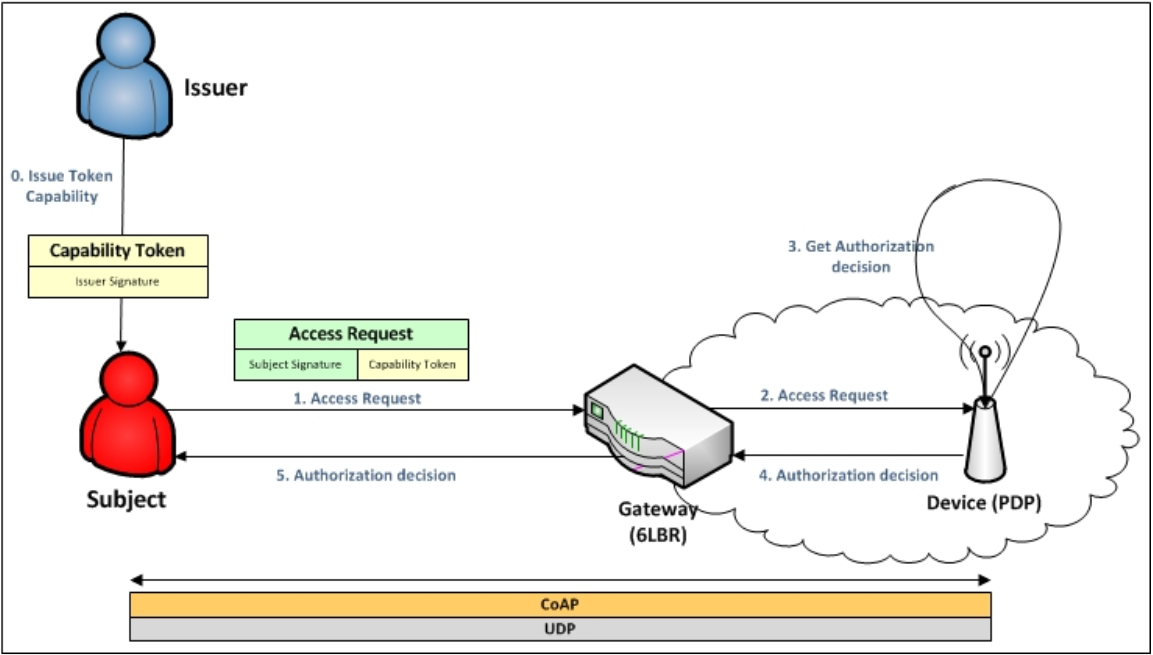
\includegraphics[scale = 0.2]{img/capBac}
\caption{CapBAC Architecture }
\label{fig:capbac}
\end{figure}

CapBAC uses ECDSA (Elliptic Curve Digital Signing Algorithm) to authenticate capability tokens and end device requests, for which all issuers and subjects are setup with an ECDSA key pair. A subject sends the request for access to a resource on an end device to an issuer, and an issuer validates and produces a capability token for this subject as a JSON file, and then signs it with its private key from it's ECDSA key pair, the subject now can sign the token with its own private key and forwards the token and it's signature to the end device. The end device first verifies the signature against the public key for the subject (\textbf{SU}) from the token, thus validating that the request did genuinely arrive from the source that is granted the capability, and then verifies that the token itself originates from a valid issuer by verifying the signature (\textbf{SI}) in the token, against the public key of the Issuer (\textbf{IS}).

CapBAC clearly uses the type of capability system with tag bits, and offers an intuitive and efficient mechanism for access control in the Internet of Things setting, however it would have been useful if CapBAC could have provided performance measures as being a generic framework for introducing capabilities, a performance evaluation on it could validate the performance for any general application.  However the original work, merely accounted the time taken for one resource access.

